%%%%%%%%% PROJECT DESCRIPTION  -- 15 pages (including Prior NSF Support)

\required{Project Description}
\begin{center}
%\emph{Maximum of 15 pages}
\end{center}
%The Project Description (including Results from Prior NSF Support, which is
%limited to five pages) may not exceed 15 pages. Visual materials, including charts,
%graphs, maps, photographs and other pictorial presentations are included in the
%15-page limitation. PIs be cautioned that the project description must
%be self-contained and that URLs that provide information related to the proposal
%should not be used. \\
%
%All proposals to NSF are reviewed utilizing the two merit review criteria,
%intellectual merit and broader impacts. \\
%
% The Project Description should provide a clear statement of the work 
% to be undertaken and must include: objectives for the period of the proposed 
% work and expected significance; relation to longer-term goals of the PI's 
% project; and relation to the present state of knowledge in the field, 
% to work in progress by the PI under other support and to work in progress 
% elsewhere.

%%%%%%%%%%%%%%%%%%%%%%%%%%%%%%%%%%%%%%%%%%%%%%%%%%%%%%%%%%%%%%%%%%%%%%
%INTRO
%%%%%%%%%%%%%%%%%%%%%%%%%%%%%%%%%%%%%%%%%%%%%%%%%%%%%%%%%%%%%%%%%%%%%%
\section*{Introduction}

While the potential role of hybridization and introgression as agents of evolution has long been postulated \citep{Anderson1948, Anderson1954, Stebbins1959}, only recently have technological innovations allowed for characterization of these processes on a genome-wide scale.
Multiple studies have now reported evidence of inter-taxon introgression in both plant \citep{Hufford2013, renaut2013} and animal \citep{consortiumbutterfly2012, staubach2012, huerta2014} species based on full-genome data.
Genomic tools provide the capacity to evaluate the genomic extent of introgression, differentiate neutral from adaptive introgression, and evaluate whether distinct hybrid populations show convergent patterns of introgression.
With this expanded perspective, we can fully evaluate hypotheses first articulated by \citet{Anderson1954}: that 1) Evolution can occur rapidly through selection on novel variation generated by hybridization, and 2) The redistribution of previously isolated species through anthropogenic activity has provided ample opportunity for hybridization to occur \citep{Anderson1954}.
Given its evolutionary history and genomic resources, the \emph{Zea} study system presents an unparalleled opportunity to test these hypotheses and realize the promise of genomic data for hybridization studies.

The genus \emph{Zea} includes four species. The annual \emph{Zea mays} consists of four subspecies: the domesticated ssp. \emph{mays}, the Mexican taxa ssp. \zp{} and ssp. \zm{} and the Guatemalan ssp. \zh. \emph{Zea luxurians} (including the populations sometimes referred to as \emph{Zea nicaraguensis}) is an annual, flood-tolerant species found in Guatemala, Honduras, and Nicaragua. 
Finally, the diploid \emph{Zea diploperennis} and its autotetraploid derivative \emph{Zea perennis} are perennial species narrowly distributed along the mountain slopes of western Mexico. 
The wild taxa, collectively referred to as teosintes, are all relatively closely related, and thought to have diverged only within that last few hundred thousand years \citep{Ross-Ibarra2009a}. 
In the investigation proposed here, we will build upon our previous work in maize (\emph{Zea mays} ssp. \emph{mays}) and its wild relatives the teosintes (\emph{Zea} spp.) to characterize the evolutionary role of hybridization and introgression in this system. 

First, analysis of hybridization in two parapatric and uniquely-adapted teosinte subspecies will allow us to answer questions about the extent to which selection determines patterns of gene flow and whether introgression is convergent across independent hybrid zones.
Second, evaluation of introgression between maize and teosinte outside the domestication center will inform our understanding of the importance of adaptive introgression during colonization of novel environments and test the role of widespread species to act as bridges for gene flow among their congeners.

This proposal builds considerably upon a previous full submission to the 2014 NSF-DEB competition that was favorably reviewed but not funded due to concerns over certain aspects of experimental design that we have rectified here.
In addition, over the last year we have conducted additional preliminary analyses, solidified collaborations with colleagues in Mexico and Guatemala, and ensured that this project is logistically feasible.

%%%%%%%%%%%%%%%%%%%%%%%%%%%%%%%%%%%%%%%%%%%%%%%%%%%%%%%%%%%%%%%%%%%%%%
%OBJECTIVES
%%%%%%%%%%%%%%%%%%%%%%%%%%%%%%%%%%%%%%%%%%%%%%%%%%%%%%%%%%%%%%%%%%%%%%
\section*{Objectives}
\subsection*{Objective I: Assess the evolutionary role of hybridization in a naturally occurring teosinte hybrid zone}
\emph{Zea mays} ssp. \emph{parviglumis} (the wild progenitor of maize; hereafter, \zp) and \emph{Zea mays} ssp. \emph{mexicana} (hereafter, \emph{mexicana}) diverged approximately 60,000 BP \citep{Ross-Ibarra2009a} and have parapatric distributions: while \zp\ occurs in the warm lowlands of southwest Mexico, \zm\  is found in the cool highlands of the Central Plateau. 
Narrow regions of admixture between these wild subspecies have been discovered at middle elevations \citep{Fukunaga2005, Pyhajarvi2013}. 
Through targeted collections, high-density genotyping, population genomic analyses, and common garden experiments, we will address the following research questions: 

\begin{enumerate}
\item \emph{Do hybrid populations show higher fitness than parental subspecies in some environments?}
\item \emph{Do independent hybrid zones show convergent patterns of introgression?}
\item \emph{Is there evidence of selection on putatively adaptive phenotypes across hybrid zones?}
\end{enumerate}

\subsection*{Objective II: Determine the extent to which anthropogenic movement of maize has enabled hybridization among taxa in \emph{Zea}}
Maize was domesticated in southwest Mexico from \zp{} $\sim$9,000 BP \citep{Matsuoka2002} and quickly spread throughout the Americas, bringing it into contact with other teosinte taxa.
Hybridization has been observed between maize and each of these teosintes, raising questions about the interaction between colonization and hybridization.
Our population genetic analysis will assess the following questions:
\begin{enumerate}
\item \emph{Does the potential for adaptive introgression depend on divergence?}
\item \emph{Is introgression adaptive across multiple spatial scales?}
\item \emph{Can a widespread species serve as a bridge for introgression among allopatric species?} 
\end{enumerate}

%%%%%%%%%%%%%%%%%%%%%%%%%%%%%%%%%%%%%%%%%%%%%%%%%%%%%%%%%%%%%%%%%%%%%%
%RATIONALE AND SIGNIFICANCE
%%%%%%%%%%%%%%%%%%%%%%%%%%%%%%%%%%%%%%%%%%%%%%%%%%%%%%%%%%%%%%%%%%%%%%
\section*{Rationale and Significance} 
Pioneers in evolutionary biology including G. Ledyard Stebbins and Edgar Anderson recognized the important role hybridization and introgression could play in adaptation and speciation \citep{Anderson1948, Anderson1954}.
These evolutionary forces were thought to be particularly influential when environmental conditions encountered by a species were marginal, variable, or new \citep{Stebbins1959}.
More recently, defined and stable regions of hybridization, referred to as hybrid zones, have been discovered in a number of taxa \citep[reviewed in ][]{HarrisonHybridZone, shurtliff2013, abbott2014}. 
It is increasingly clear that the phenomena of hybridization and subsequent introgression shape genomes and influence the trajectory of species as they evolve \citep{Ellstrand2014}.
Hybridization has long been believed to play a role in speciation, and introgression of even a small number of loci can enable a species to adapt and invade novel habitats \citep{currat2008, abbott2013}.
For example, we now have strong molecular evidence that hybridization has led to speciation in both plants and animals \citep[reviewed in][]{mallet2007} and that colonization events of non-native species \citep{lucek2010} and domesticated crops \citep{he2011, Hufford2013} have been facilitated by introgression. 

While theory regarding hybridization has progressed and many compelling empirical examples have been identified, several outstanding questions remain. 
For example, are hybrid zones largely maintained by adaptive or purifying selection or strictly neutral processes \citep{Kruuk1999, Rasmussen2012, Smith2013b}? 
If introgression is adaptive, what is the geographic scale of this adaptation?
Are the same adaptive alleles introgressed across independent hybrid populations or are patterns of introgression driven more by local environmental conditions?
Can a widespread congener act as a bridge for gene flow between more narrowly distributed allopatric taxa?
Genome-wide analysis of variation in the extent and genetic architecture of introgression --- the number and size of introgressed loci ---  will offer considerable insight regarding each of these questions.  
For example, the few genomic studies of introgression completed thus far have already suggested that rates of gene flow vary substantially across loci, likely as a function of selection on introgressed alleles \citep{Hufford2013, Poelstra2014} and that introgression has occurred at genomic locations underlying adaptive phenotypes that may have facilitated colonization of a non-native taxon \citep{Hufford2013}.
As described below, the \emph{Zea} study system is uniquely suited to address remaining, timely questions in the field of hybridization biology from a genome-wide perspective.

%%%%%%%%%%%%%%%%%%%%%%%%%%%%%%%%%%%%%%%%%%%%%%%%%%%%%%%%%%%%%%%%%%%%%%
%SPECIFIC OBJECTIVES
%%%%%%%%%%%%%%%%%%%%%%%%%%%%%%%%%%%%%%%%%%%%%%%%%%%%%%%%%%%%%%%%%%%%%%
\section*{Research Plan}

%\subsection{OBJECTIVE}
%background paragraph on relevant biology
%\subsubsection{A}
%paragraph describing hypotheses and predictions
%paragraphs explaining what we're gonna do
%\subsubsection{B}
%paragraph describing hypotheses and predictions
%paragraphs explaining what we're gonna do
%\subsubsection{C}
%paragraph describing hypotheses and predictions
%paragraphs explaining what we're gonna do
%\subsubsection{Prelim Results}
%What data we have so far
%\subsubsection{Potential Challenges}
%not interpretation of hypotheses but explicitly what if something goes wrong what we do.

%OBJECTIVE ONE%%%%%%%%%%%%%%%%%%%%%%%%%%%%%%%%%%%%%%%%%%%%%%%%%%%%%%%%%
\subsection{Assess the evolutionary role of hybridization in naturally occurring teosinte hybrid zones}
\label{ss:hybrids}

The \emph {Zea mays} subspecies \emph{parviglumis} and \emph{mexicana} are distributed across a steep elevationnal gradient and differ for phenotypes that are thought to be adaptive in the highlands such as the presence of macrohairs, stem pigmentation and shorter flowering time in \emph{mexicana}.
A recent ecological niche study has found that the potential distributions of these subspecies are largely allopatric and stable over many thousands of years \citep{hufford2012inferences}.
However, analysis of microsatellite markers genotyped in a large sample of the two subspecies suggested elevated admixture between them in mid-elevation regions of Mexico where their distributions overlap, potentially indicating the presence of a hybrid zone \citep{Fukunaga2005}.  
Our recent genome-wide analysis of twelve individuals from one such population revealed abundant small blocks of admixture in all individuals, suggesting long-term gene flow between subspecies \citep{Pyhajarvi2013}.  
Very little is known, however, about patterns of introgression across populations in this region.

To further refine our research questions and provide preliminary results for this proposal we have reanalyzed published data \citep{Fang2012} of 983 SNPs genotyped across a panel of $>2,000$ samples including all subspecies and species of teosinte and an Americas-wide sample of maize landraces (\emph{i.e.}, traditional open-pollinated varieties).
While the low density of markers in these data precludes genome-wide inferences and haplotype-based analyses, the comprehensive taxon sampling makes this an ideal resource for guiding future research.
\begin{figure}[t] 
  \centering
   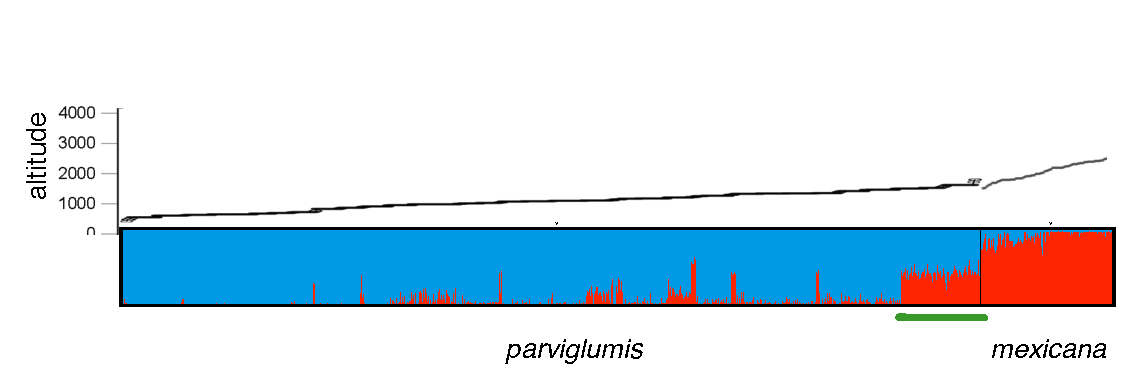
\includegraphics[width=0.95\textwidth]{structure.pdf}
    \caption{Assignment of \emph{parviglumis} and \emph{mexicana} individuals to K=2 groups using the Bayesian assignment algorithm of STRUCTURE \citep{Pritchard2000}.  Individuals are sorted by increasing elevation as indicated by the plot above the bar chart. Individuals from mid-elevation, hybrid zone populations are underscored in green.} 
\label{fig:structure}
\end{figure}
Using these data we calculated the probability of assignment of samples to \emph{parviglumis} and \emph{mexicana} groups with the program STRUCTURE \citep{Pritchard2000}.  We find that individuals from several mid-elevation populations show appreciable assignment to both groups (Figure \ref{fig:structure}) and likely represent hybrid populations.  
Admixed populations cluster in two geographically distinct regions of Mexico: the eastern Balsas River Basin and eastern Jalisco state.
These locations fall at intermediate locations between the main distributions of \emph{parviglumis} and \emph{mexicana} (Panel A, Figure \ref{fig:pies}).
Hybrid populations from eastern Jalisco state are found at higher elevation (mean 1632m) than those in the eastern Balsas (mean 1531m) and also show a higher proportion of membership in the highland teosinte \emph{mexicana} group (Panels B and C, Figure \ref{fig:pies}).
These findings suggest that hybrid populations from distinct environments may vary in the proportion of ancestry from each subspecies in a manner that is adaptive.
Estimates of pairwise population differentiation ($F_{ST}$; data not shown) also suggest that hybrid populations in the Balsas and Jalisco are distinct in that Jalisco populations are less differentiated from \emph{mexicana} than hybrid populations in the Balsas.  Not surprisingly, populations in both hybrid zones are less differentiated from \emph{mexicana} and \emph{parviglumis} than these subspecies are from each other.
Finally, we have grown plants from populations in both the Jalisco and Balsas hybrid zones in smallscale growth chamber experiments and have found that they have intermediate morphologies between \zp{} and \zm{}.

\begin{figure}[h!]
  \centering
   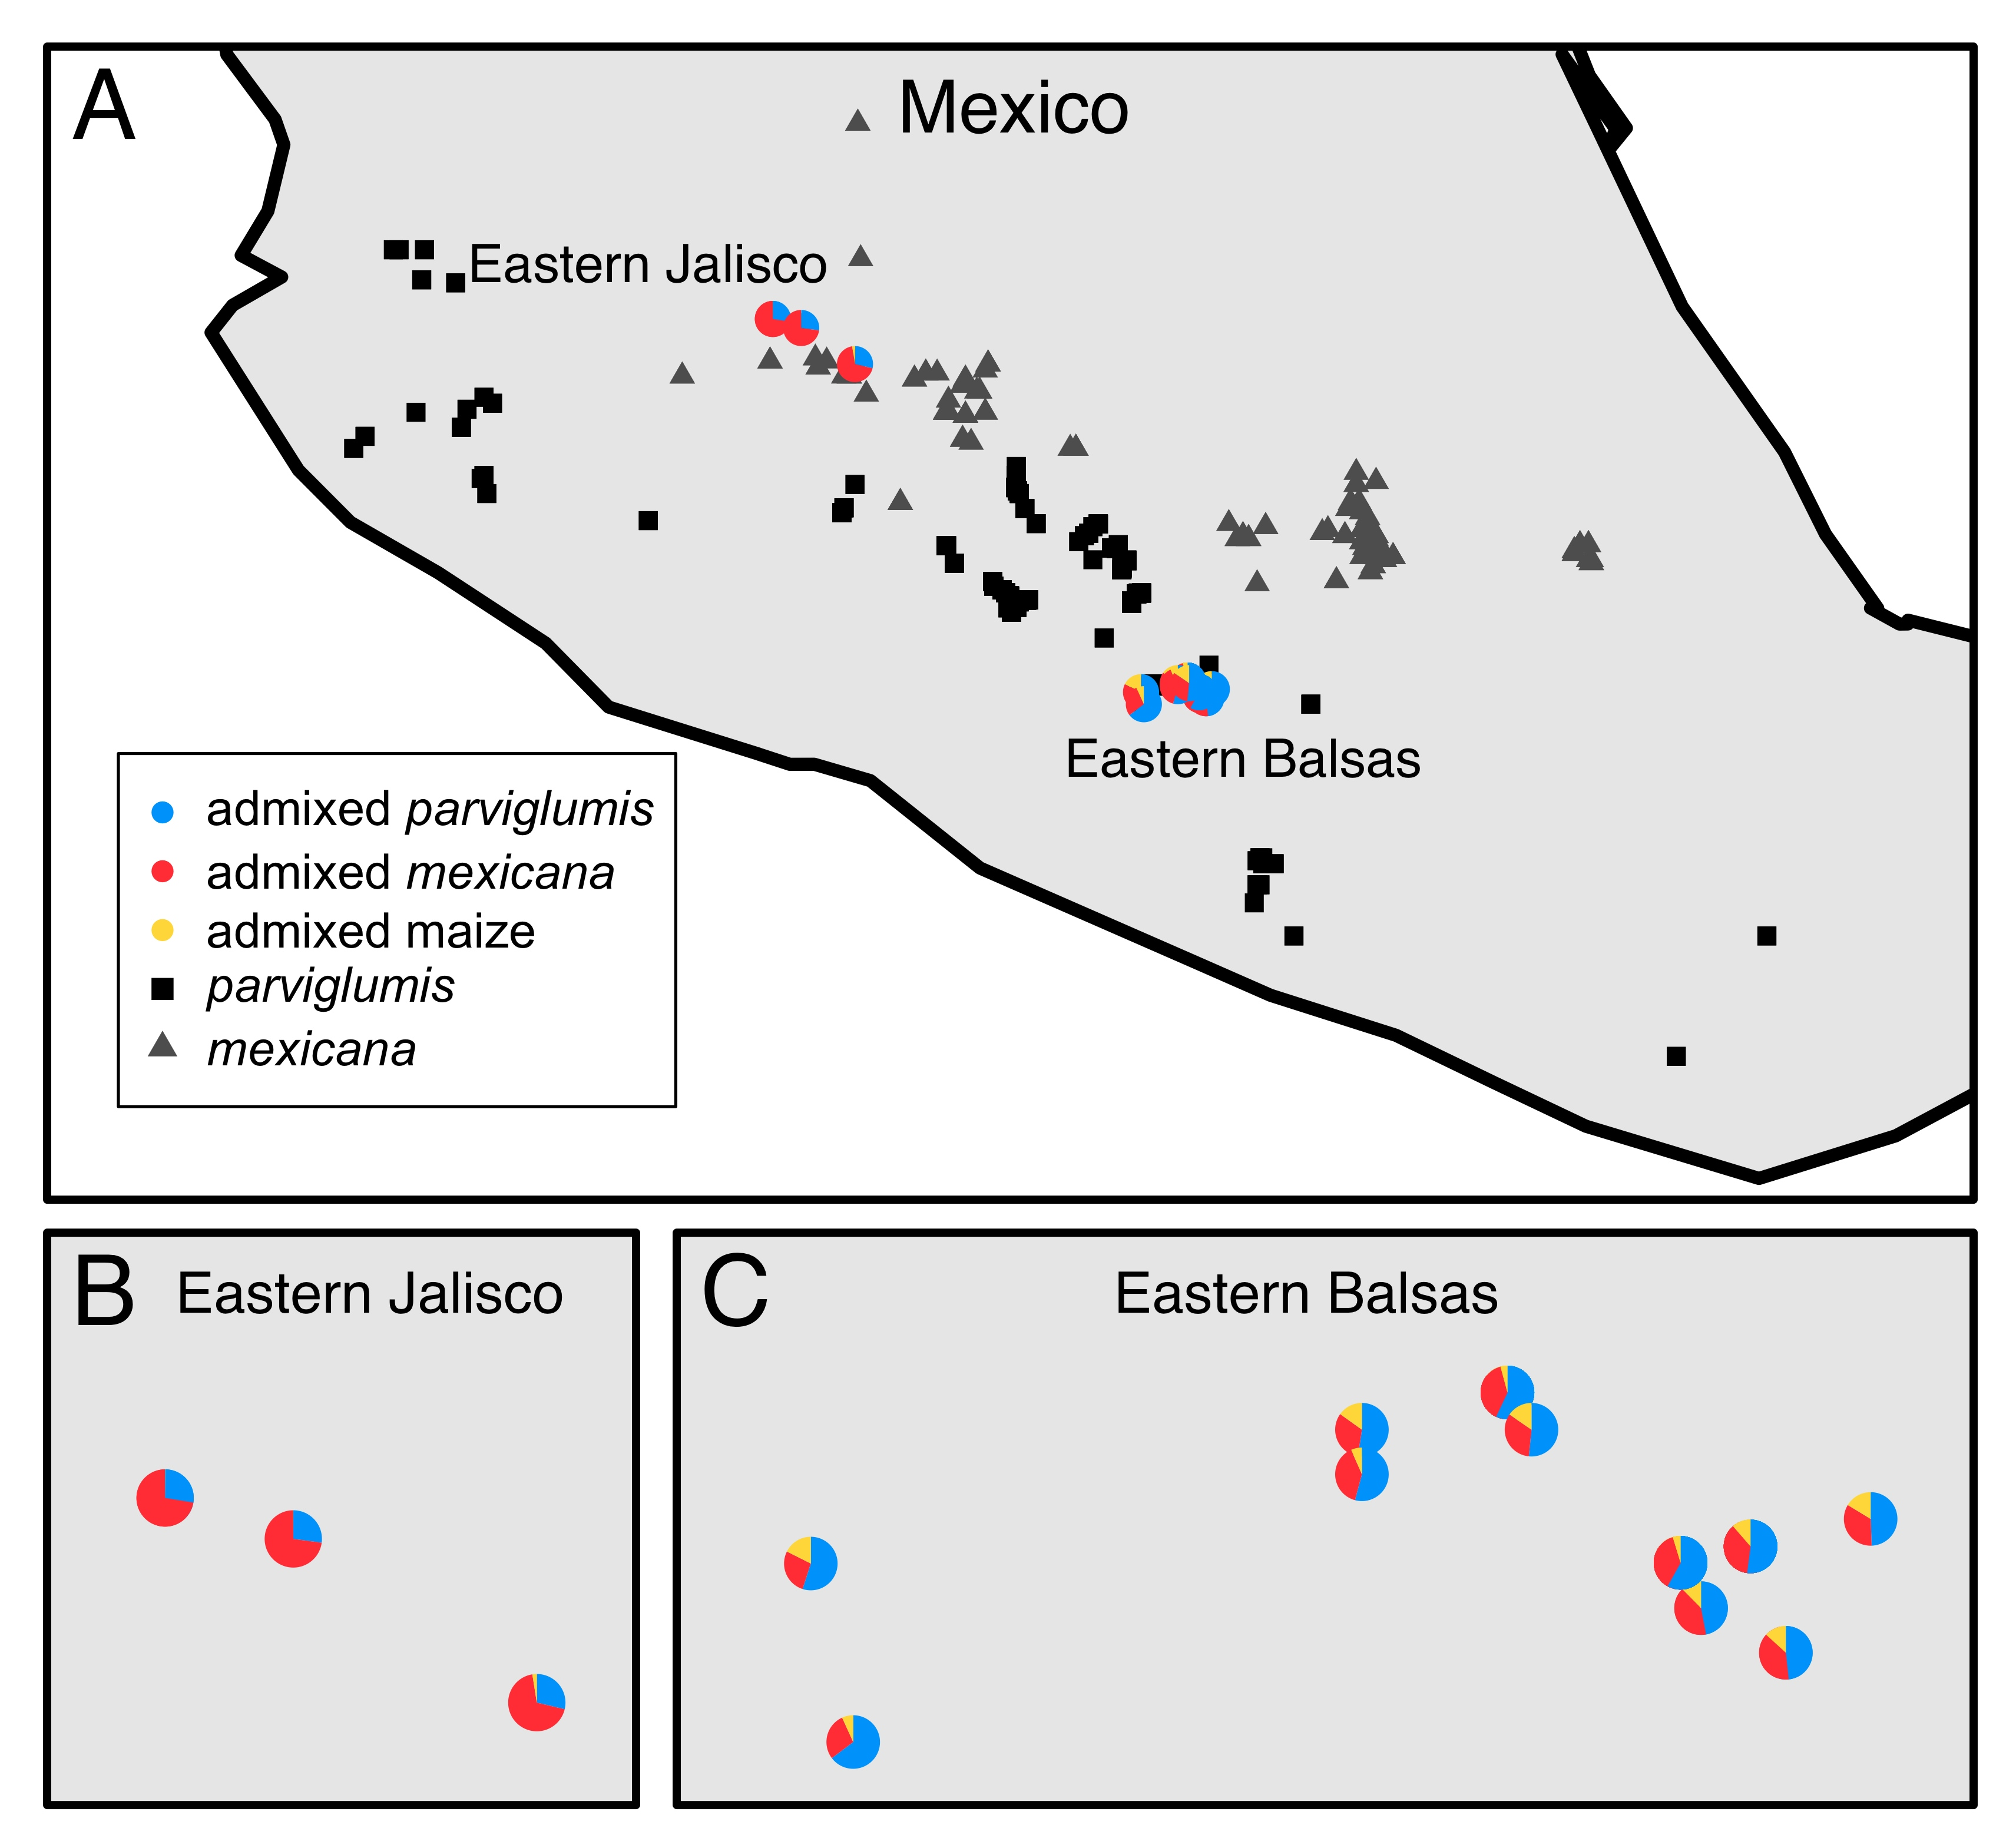
\includegraphics[width=0.7\textwidth]{Figure1.jpg}
    \caption{A) Location of two putative hybrid zones of \emph{mexicana} and \emph{parviglumis}.  Hybrid populations are represented as pie charts with proportion assigned to \emph{mexicana}, \emph{parviglumis}, and maize groups. Zoomed-in views of the Eastern Jalisco (B) and Eastern Balsas (C) hybrid populations.} 
\label{fig:pies}
\end{figure}

Few studies have gauged evidence for selection and dissected the genome-wide architecture of hybridization in replicate hybrid zones.
The Hufford Laboratory and Senior Personnel Luis Eguiarte will investigate these questions in two hybrid zones of \zm{} and \zp{} through targeted collections, generation of phenotype, genotype and genome sequence data, and application of quantitative and population genetic analyses as described in the following three sub-objectives.

%HYBRID FITNESS%%%%%%%%%%%%%%%%%%%%%%%%%%%%%%%%%%%%%%%%%%%%%%%%%%%%%%%%%
\subsubsection{Do hybrid populations show higher fitness than parental subspecies in some environments?} 
\label{sss:fitness}

Currently, there are two dominant hypotheses amongst evolutionary biologists for the stability of hybrid zones over time: the tension zone and the bounded hybrid superiority zone (\emph{i.e.,} ecotone) hypotheses.
Under tension zone dynamics hybrids have lower fitness relative to their parental taxa across environments due to, for example, incompatibility factors that arise when divergent taxa mate.
Tension zones arise at the interface of parental taxa and are typically narrow clines due to the effects of purifying selection \citep{abbott2014}.
In contrast, under ecotone dynamics hybrids have a selective advantage in intermediate environmental conditions relative to parental species and their distribution is typically characterized as a smooth transition between parental habitats \citep{abbott2014}.
Hybrid populations of \zp{} and \zm{} span several kilometers (Figure \ref{fig:pies}) under environmental conditions intermediate to their parental taxa suggesting ecotone dynamics prevail.
We will test this hypothesis by assessing fitness and variation at putatively adaptive phenotypes across both non-admixed and hybrid populations in common garden experiments conducted in Mexico at three elevations: 1) Below a hybrid zone in habitat occupied by non-admixed \emph{parviglumis}; 2) Within hybrid zone habitat; and 3) Above a hybrid zone in habitat occupied by non-admixed \emph{mexicana}. 

From previous collections, we have access to extensive sampling of \zm{} and \zp{}.
Moreover, Senior Personnel Luis Eguiarte has recently collected altitudinal transects of \zp{} and \zm{} that extend through both hybrid zones we have identified \citep{Diez2013} and is familiar with populations in this region.
However, our current collections will need to be expanded in order to conduct the activities we propose and we have therefore budgeted for a collection trip during the first year of the project.
We will collect from 15 sampling sites in each of 16 populations (four non-admixed populations each of \zp{} and \zm{} and four populations from both hybrid zones).
Sampling sites will be randomly stratified across the elevation gradient of each population.
At each sampling site we will collect as much seed as possible from each of five teosinte plants (in the wild, teosinte plants produce an average of $\sim$100 seeds per plant \citep{wilkes1967teosinte}). 
While elevation and correlated trends in temperature and precipitation appear most important in patterning the distribution of hybrids, we will also collect local environmental data at each sampling site including plant density (in 1 $m^2$ quadrats), slope of the terrain, and canopy cover.
A single soil sample will also be collected from each population.  
We have already obtained the requisite collection permits as well as permits for importing samples into the United States for the genetic analyses proposed in \ref{sss:genomescan}.

Following collection, samples will be sent to Irapuato, Mexico for seed increase (see letter of support from our collaborator Ruairidh Sawers at Langebio in Irapuato).
Irapuato is a mid-elevation site and will be best-suited for increasing seed from all populations in a single environment.
Forty-five plants per population (three from each sampling site) will be grown in isolated plots surrounded by a detasseled maize buffer and will be allowed to open-pollinate.
Seed will be harvested from each plant, keeping each plant's seed separate in order to preserve half-sibling relationships that are necessary for the $F_{ST}$--$Q_{ST}$ framework used in \ref{sss:driftsel}.
This single generation of seed increase in a common environment is necessary to remove maternal effects that may confound phenotypic comparisons of populations in our common garden experiments.

Common garden experiments will be replicated at three sites along an elevation gradient during years two and three of our proposed project.
Our lowland site is outside of Bucerias, Nayarit state (40m), our mid-elevation site is in Irapuato, Guanajuato state (1700m), and our highland site is in Metepec, Mexico state (2600m).
We have experience working in these sites and have confirmed that our common gardens will be logistically feasible.
Each garden will consist of three complete blocks including a randomization of a half-sibling family from each sampling site of our 16 sampled populations (3 blocks x 3 half siblings per sampling site x 15 sampling sites x 16 populations = 2,160 plants per garden).  
We will measure fitness-related phenotypes (percent germination, germination rate, plant height at 15-day intervals, total seed set, 50-seed weight, total-above-ground biomass, stomatal conductance and survival), putatively adaptive phenotypes across the altitudinal gradient (macrohair density, pigmentation extent, and flowering time) and a phenotype for which there is no \emph{a priori} evidence of selection across an elevational gradient (the width of the leaf beneath the first lateral branch at the time of flowering).  

Comparison of fitness of hybrid and parental plants across our garden sites will provide evidence regarding ecotone versus tension zone dynamics in teosinte hybrid zones.  Ecotone dynamics would be supported by hybrids possessing the highest fitness of all plants in the mid-elevation garden, whereas tension zone dynamics would be supported by hybrids having lower fitness in all gardens.
Phenotypic data for putatively adaptive traits and our trait with no evidence of selection will be analyzed in \ref{sss:driftsel}.

%CONVERGENCE%%%%%%%%%%%%%%%%%%%%%%%%%%%%%%%%%%%%%%%%%%%%%%%%%%%%%%%%%
\subsubsection{Do independent hybrid zones show convergent patterns of introgression?}
\label{sss:genomescan}

%\jri{convergence works regardless of above. if hybrids suck, are same loci causing DMIs?  if hybrids rock, same loci adaptively introgressed? if hybrids are good (part 1) and selection on phenotype (part 2) then lack of convergence means standing variation for quant. traits (cite Takuno!).}
While we cannot predict whether tension zone or ecotone dynamics define teosinte hybrid zones prior to completing our common garden experiments, assessment of genome-wide patterns of introgression will be an essential next step regardless of this outcome.
If we find that hybrids are selected against and exist within two discrete tension zones, then our primary interest will be in investigating the level of convergence in hybrid inviability loci (\emph{i.e.,} Dobzhansky-Muller incompatibilities) across populations and independent hybrid zones.
Should hybrid populations show superior fitness in our intermediate garden alone and follow an ecotone model, we will instead investigate convergence in the genetic architecture of adaptive introgression.

During year two of our proposed project, leaf tissue will be collected from a single plant per sampling site ($n=240$) in our mid-elevation common garden (see \ref{sss:fitness}) at the 5-7 leaf stage, stored in silica, and shipped to Iowa State University for DNA isolations, subsequent genotyping and full-genome sequencing.
DNA for genotyping will be isolated using the Qiagen DNeasy Plant Mini Kit.
For sample genotyping ($n=240$) we will utilize the services of the Genomic Diversity Facility at Cornell University to implement a reduced representation approach to next-generation sequencing called Genotyping By Sequencing (GBS; \citealt{Elshire2011}).
To date, this method has been implemented to genotype tens of thousands of maize samples and a bioinformatics pipeline (TASSLE-GBS) has been constructed that allows for genotyping $\sim$1,000,000 SNPs in maize \citep{Glaubitz2014} using standard GBS data. 
We will multiplex only 48 individuals per lane (instead of the standard 384 used for inbred lines) to minimize missing data and errors in identifying heterozygous genotypes. 
Based on our experience with diverse maize and teosinte \citep[\emph{e.g.,}][]{Takuno15062015, mezmouk2014pattern}, even after filtering for missing data, GBS provides many more markers with minimal ascertainment bias at a fraction of the cost of other available technologies. 

In addition to GBS data, we will generate full-genome sequence through the Iowa State University DNA Facility for a single hybrid individual from each hybrid zone.  We will generate two lanes of Illumina HiSeq 150bp, paired-end data per individual. 
We have previous experience dealing with whole genome shotgun data \citep{Gore2009, Chia2012a,  Hufford2012b, da2015origin}, and have recently developed and implemented an open-source pipeline for read-mapping and SNP calling (\url{https://github.com/RILAB/paap}) using the existing maize B73 reference genome. 
 
We will assess genome-wide patterns of ancestry (\zp{} versus \zm{}) in hybrid individuals using several approaches.  
First, standard measures of differentiation including $F_{ST}$, the proportion of shared and fixed variants, and relative levels of nucleotide diversity \citep{Geneva2014} will be calculated in sliding windows along the genome. 
These will be complemented by window-based methods using counts of derived alleles \citep{martin2015evaluating}.
Second, we will implement haplotype-based methods for detecting introgression \citep[\emph{e.g.},][]{price2009, lawson2012} that will effectively allow us to model chromosomes from hybrid populations as mosaics of our allopatric reference populations of \emph{parviglumis} and \emph{mexicana}.  

We will evaluate \emph{parviglumis} and \emph{mexicana} ancestry on a site-by-site basis across each hybrid genome and determine level of convergence at three levels: individual, population, and independent hybrid zone.  
Chromosomal regions showing an excess of ancestry from one taxon in hybrid populations will be inspected for evidence of selection using a combination of site-frequency-, linkage-disequilibrium-, and population-differentiation-based methods \citep[reviewed in][]{Vitti2013}.
Chromosomal regions showing strong evidence of selection across individuals within a hybrid zone based on analysis of GBS data will be inspected in our whole-genome resequencing data to refine haplotype boundaries. 
Whole genome sequence data will also allow estimation of the age of the introgression and, potentially, the identification of candidate causal polymorphisms.



%PHENOTYPE SELECTION%%%%%%%%%%%%%%%%%%%%%%%%%%%%%%%%%%%%%%%%%%%%%%%%%%%%%%%%%
\subsubsection{Is there evidence for selection on putatively adaptive phenotypes across hybrid zones?}
\label{sss:driftsel}
\jri{background then hypotheses here. change focus to selection {\bf in hybrid pops}. then build on part 1: if hybrids higher fitness we should see selection on phenotypes. if hybrids suck, adaptive phenos show no selection (or selection in wrong direction?)}

Stem pigmentation, macrohair density, and flowering time in particular are thought to be under selection in teosinte across an elevational gradient.  Pigmented and pilose plants have an advantage in retaining heat at high elevation (for a discussion of highland adaptation in the context of maize see \citealt{Eagles1994}). Additionally, \emph{mexicana} flowers much earlier than \emph{parviglumis} \citep{Rodriguez2006}, which may represent an adaptation to shorter growing seasons at high elevation. We will combine our genome-wide marker data obtained in \ref{sss:genomescan} with phenotypic data collected in our common garden experiments in \ref{sss:fitness} in order to evaluate evidence for selection on these potentially adaptive phenotypes.  A method recently developed by \citet{Ovaskainen2011} and implemented in the software DRIFTSEL \citep{Karhunen2013} is particularly suited to this purpose.  The method builds upon the $F_{ST}$--$Q_{ST}$  framework for comparison of population differentiation and quantitative phenotype divergence and allows the signature of selection on a given phenotypic trait to be distinguished from genetic drift.  The strength of evidence for selection based on DRIFTSEL for putatively adaptive phenotypes (pigment, macrohairs, flowering time) will be compared to that of phenotypes with no \emph{a priori} evidence of selection across an elevational gradient (culm diameter and leaf width). 

In addition, we will conduct association analyses to connect genotype to phenotype using GBS data described in \ref{sss:genomescan} and phenotypic data for potentially adaptive traits and traits gauging fitness.  Association analysis will be conducted using TASSEL5.0 \citep{Bradbury2007}. Significant associations will then be cross-referenced with regions of excess ancestry from \emph{parviglumis} or \emph{mexicana} in hybrid populations and zones identified in \ref{sss:genomescan}, particularly those that show evidence of selection based on additional population genetic summary statistics.  This final combination of data and analyses could reveal the phenotypes, loci, and ancestry source under selection within hybrid zones.

\paragraph{\emph{Preliminary Results:}} 
\jri{add here prelim growth chamber expers. that suggest hybrids better than parents in some pops.}

\paragraph{\emph{Potential Challenges:}}
\jri{add here that if field collects not work, we already have smaller sets of seed from hybrid pops collected by collabs}

Some of the population-genetic analyses proposed may have difficulty with the high rate of missingness and heterozygous error in GBS data.
If these approaches do not work or force us to remove too much of our data, we will instead take advantage of approaches designed  to estimate admixture from genotype-likelihoods calculated on low-coverage sequence data \citep{skotte2013estimating}. 
We have already designed pipelines to work with genotype-likelihoods (e.g. \url{https://github.com/arundurvasula/angsd-wrapper}) and can utilize these methods to calculate standard diversity statistics as well.  

%OBJECTIVE TWO%%%%%%%%%%%%%%%%%%%%%%%%%%%%%%%%%%%%%%%%%%%%%%%%%%%%%%%%%
\subsection{Determine the extent to which anthropogenic movement of maize has enabled hybridization among \emph{Zea} taxa} 
\label{ss:genuswide}
Following its domestication from \zp{}, maize spread rapidly across the Americas \citep{Piperno2001,Grobman2012}, colonizing novel environments distinct from that inhabited by its wild ancestor. 
As its range expanded, maize came into contact with other wild teosinte that had been allopatric to \zp{} for long periods prior to domestication \citep{hufford2012inferences}.  
Hybridization between maize and each of these taxa has been documented based on morphological \citep{wilkes1967teosinte, Wilkes1977} and genetic \citep{doebley1990molecular,Fukunaga2005,Ross-Ibarra2009a,vanheerwaarden2011a} data, raising a number of questions about the role of gene flow in the recent evolution of both maize and its wild relatives.

In this objective, the Ross-Ibarra Laboratory will use population genetic approaches to address three questions that arise from this natural experiment.  
First, we will use maize and teosinte populations in Guatemala to investigate whether divergence time between taxa affects the possibility of adaptive introgression. 
Second, we will take advantage of multiple pairs of sympatric maize and teosinte populations from both Mexico and Guatemala to test hypotheses about the geographic scale of adaptive introgression.
Finally, we will use population-level comparisons of maize and all the diploid taxa in \emph{Zea} to test the hypothesis that maize has served as a bridge for gene flow between otherwise allopatric teosinte \citep{Ross-Ibarra2009a}.



%DIVERGENCE TIME%%%%%%%%%%%%%%%%%%%%%%%%%%%%%%%%%%%%%%%%%%%%%%%%%%%%%%%%%
\subsubsection{Does the potential for adaptive introgression depend on divergence?}
\label{sss:adaptive_intro}
Most models of speciation predict that introgression between taxa should decrease with increasing divergence between them \citep{harrison2014hybridization}, as differences contributing to postzygotic isolation are expected to increase as the square of divergence time \citep{orr2001evolution}. Maize colonization of novel environments in Guatemala that are inhabited by distinct teosinte species offers an opportunity to test the importance of divergence in restricting the potential for adaptive introgression.

Following domestication, maize spread southward into Guatemala into conditions distinctly more tropical than those found in its center of origin in southwest Mexico.
In comparison to southwest Mexico, Guatemalan winters are warmer, annual fluctuation in temperature is lower, and there is nearly double the annual precipitation.
Upon arrival in Guatemala, maize came into contact with two new teosintes \emph{Zea mays} ssp. \emph{huehuetenangensis} (hereafter, \emph{huehuetenangensis}) and \emph{Zea luxurians} (hereafter, \emph{luxurians}). 
Both teosintes exhibit a number of adaptations to tropical environments including differences in root architecture, flooding tolerance, and delayed flowering \citep{wilkes1967teosinte, mano2006}.
Hybrids between maize and both taxa \citep{wilkes1967teosinte} have been observed, providing the opportunity for adaptive introgression.  

If divergence impacts the potential for adaptive introgression, we predict different patterns of maize-teosinte hybridization for each of these taxa. 
Divergence time between maize and \zh{} is not known, but it has been classified as a subspecies of \emph{Zea mays} \citep{doebley1990systematics} and we predict that adaptive introgression from \zh{} is likely, as we have previously observed from subspecies \zm{} \citep{Hufford2013}.
\emph{Zea luxurians}, however, exhibits a number of morphological differences from \emph{Zea mays} \citep{doebley1980taxonomy}, has a much larger genome \citep{tenaillon2011genome}, and divergence time between the two taxa has been estimated at $\sim$150,000 generations \citep{Ross-Ibarra2009a}. 
Although 150,000 generations is not extremely long, it is more than twice the divergence time between maize and \zm{}, yet \zm{} has already evolved several loci which confer post-mating prezygotic isolation from maize \citep{evans2001teosinte,kermicle2010zea,kermicle2006gametophyte}.
Prezygotic isolation mechanisms in plants are not thought to evolve more rapidly than postzygotic factors \citep{widmer2009evolution}, and we thus predict that the increased genetic divergence from \zl is sufficient to lead to decreased gene flow with maize. 
If we do observe adaptive introgression, these ideas predict it will nonetheless be at fewer loci due to potential linkage with incompatibility factors. 
Because gene flow from colonizing, domesticated maize is likely to be maladaptive \citep{Hufford2013}, we also predict decreased introgression from maize into both  teosinte taxa. 
Though incompatibilities are expected to be stronger in \zl{}, this species also has a relatively low effective population size \citep{Ross-Ibarra2009a} and selection against maladaptive introgression may be less efficient.
Evidence supporting this possibility comes from the observation of alleles diagnostic of highland Mexican maize both in Guatemalan maize (Figure \ref{fig:inv4mmap}) and \zl{} samples from Guatemala \citep{Fang2012}.

\begin{SCfigure}[][t]
  	\centering
  	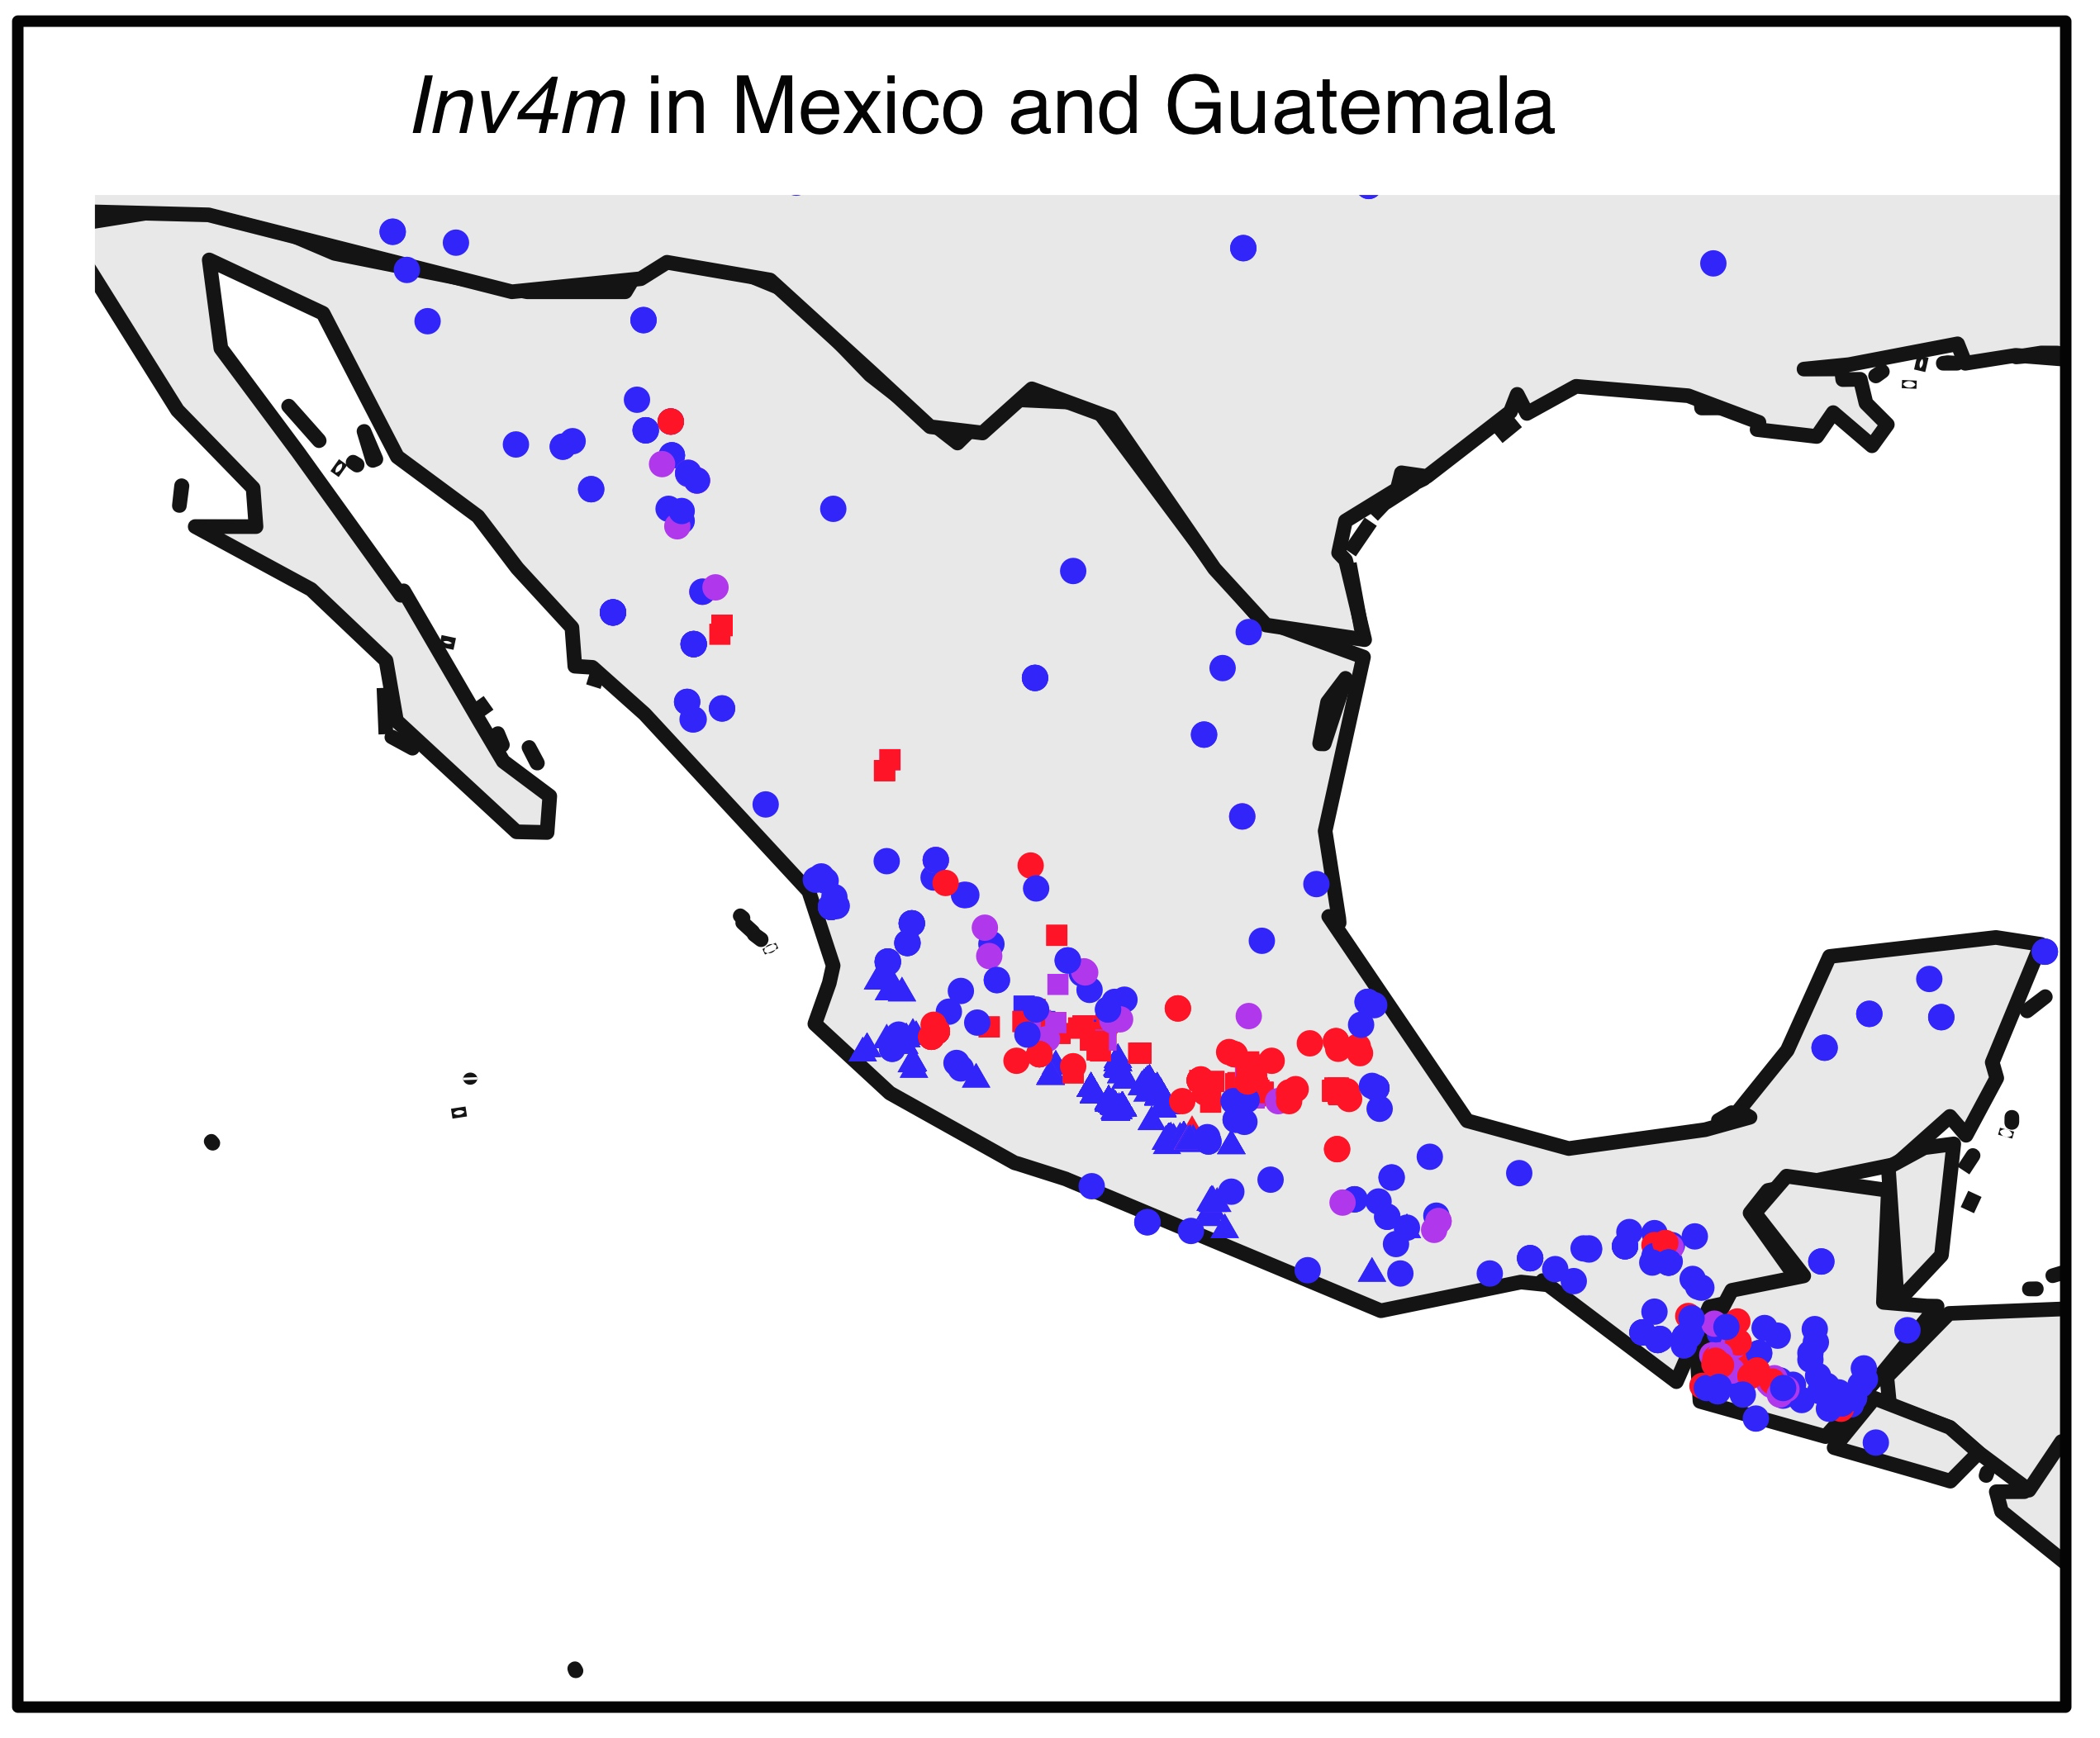
\includegraphics[width=0.5\textwidth]{inv4m_lux}
  	\caption{Geographic distribution of alleles at a SNP diagnostic of the highland maize  inversion \emph{Inv4m}.  Genotypes are shown in color (blue: homozygous standard, purple: heterozygous, red: homozygous inverted) and shapes represent taxa (squares: \zm, triangles: \zp, circles: domesticated maize). Data from \citet{Fang2012}  } 
	\label{fig:inv4mmap}
\end{SCfigure} 

To test our predictions about the role of divergence time, the Ross-Ibarra Laboratory, in collaboration with Senior Personnel Claudia Calderon, will sample six populations each of \zl{} and \zh{} stratified across their elevational range in Guatemala.  
We will sample four sympatric sites for each teosinte, collecting samples from both the maize and teosinte populations at each site.
Two populations as distant as possible from domesticated maize will be used as controls, taken to represent ancestral populations absent of admixture.  
Finally, four Guatemalan maize populations allopatric to teosinte will also sampled, for a total of 24 maize and teosinte populations.
We will be assisted in our collection by Hector Tuy of the Institute of Agriculture, Natural Resources and Environment (IARNA) in Guatemala (see attached letter of commitment).
We will genotype 12 individuals from each population using GBS (as described in \ref{sss:genomescan} but multiplexing 96 per lane), and analysis of introgression and selection will follow methods described in \ref{sss:genomescan}.  
Evaluation of the adaptive nature of observed introgressions will follow \citet{Hufford2013}, using data on QTL for putatively adaptive phenotypes \citep{omori2007qtl,mano2008linkage} and small-scale growth-chamber experiments to compare phenotype and growth rate under different conditions.

In addition to our GBS data, we will sequence one allopatric and one sympatric individual each of \zl{} and \zh{} to $\sim30X$ using paired-end 150bp reads on an Illumina Hi-Seq 3000; no deep whole-genome sequence currently exists for either taxon.
Combined with our existing, high-depth landrace maize sequences (see Preliminary Results), these sequences will allow additional tests of introgression, refine introgressed or selected regions and potentially identify candidate adaptive polymorphisms within the regions of interest.

These analyses will test the role of divergence time in limiting the potential for adaptive introgression and help establish whether observations of adaptive introgression from crop wild relatives may be a common occurrence that has facilitated the spread of domesticated taxa beyond their original habitat.
The results will also provide useful baseline information on patterns of genetic diversity in two teosinte taxa of conservation concern within Guatemala and of interest for novel root phenotypes for breeding including root angle, adventitious root formation, and the formation of aerenchyma \citep{omori2007qtl,mano2007breeding}. 

%SPATIAL SCALES%%%%%%%%%%%%%%%%%%%%%%%%%%%%%%%%%%%%%%%%%%%%%%%%%%%%%%%%%
\subsubsection{Is introgression adaptive across multiple spatial scales?}
\label{sss:scale}

Due to their sessile nature, plants must adapt to their local environments. 
The geographical scale of adaptation varies widely, however, from large portions of a species range \citep{lowry2010, fang2014} to extremely local adaptation on the scale of a few meters \citep{hamrick1979}.  
While there are now several examples of introgression facilitating colonization and adaptation (reviewed in \citealt{Bock2015}) we know little about the geographic scale at which this occurs.
Alleles that have spread throughout a wide geographic range in local populations have been tested in multiple genetic backgrounds and multiple microenvironments, and as such may have a higher likelihood of being adaptive in new populations via introgression.
In contrast, the selective benefit of alleles that are adaptive on a very local scale in a single population may depend more strongly on genetic background or particular aspects of the microenvironment and may fare worse when introgressed into a new population. 
These arguments lead us to predict that adaptive introgression across maize populations found in sympatry with teosinte will be dominated by alleles beneficial over a larger geographic area.
We should thus see parallel patterns across most populations, with relatively few loci showing evidence of adaptive introgression only in one population.
Consistent with this prediction, our previous analysis of adaptive introgression from \zm{} found highly similar patterns of introgression across all high-elevation sympatric populations, with few examples of introgressed regions at high frequency in a single population (Figure \ref{fig:sameregions}).
However, the relatively low density SNP data in our prior work provide poor resolution to identify all but the strongest selection signatures \citep{tiffin2014advances} and suffer from ascertainment bias that may limit detection of diverged haplotypes. 
  
\begin{figure}[t]
  \centering
   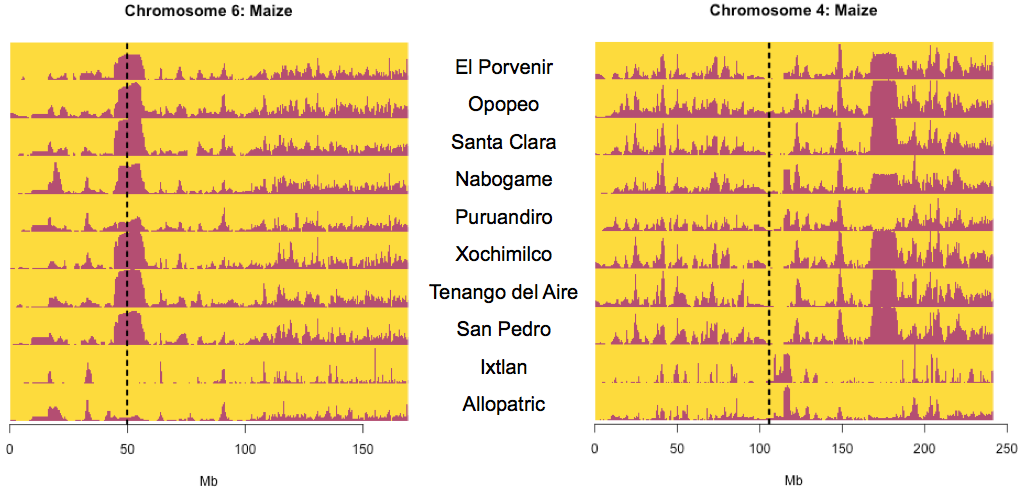
\includegraphics[width=0.75\textwidth]{same_regions}
    \caption{ Introgression from \zm\ to maize along chromosomes 4 and 6 \citep{Hufford2013}. Each row represents a population of maize, and the frequency of the \zm\ allele at a given position is shown in dark red. Consistent signals of introgression are evidence in several chromosomal regions across all populations except the two lowest elevation sympatric populations (Ixtlan and Puruandiro) and the allopatric population.}
\label{fig:sameregions}
\end{figure} 

To investigate the scale of adaptive introgression in maize, we will analyze a set of sympatric pairs of maize and teosinte populations from the highlands of Central Mexico (with \zm), the Pacific coast of Mexico (with \zp), and the humid lowlands of Guatemala (with \zl\ and \zh). 
In addition to the populations sampled in \ref{sss:adaptive_intro}, we will sample 12 maize and 12 teosinte from each of three \zm\ and \zp\ sites previously identified as sympatric with domesticated maize \citep{hufford2010genetic, Hufford2013}.  
We will endeavor to sample different environments within the range of each teosinte to maximize our opportunity to identify differential local adaptation.
Maize and teosinte individuals from each population will be genotyped using GBS, and we will test for introgression and selection following methods proposed in \ref{sss:genomescan}.
We will also make use of whole-genome resequencing data to better characterize introgressed haplotypes and identify potential candidate loci. 
Resequencing data will already be available for maize landraces (see Preliminary Results) and most teosinte (\ref{sss:adaptive_intro} and Preliminary Results), but only two low-coverage inbred \zm{} genomes are currently available \citep{Chia2012a}. 
We will thus resequence two \zm{} genomes to complement these data.

%BRIDGE%%%%%%%%%%%%%%%%%%%%%%%%%%%%%%%%%%%%%%%%%%%%%%%%%%%%%%%%%
\subsubsection{Can a widespread species serve as a bridge for introgression among allopatric species?}
\label{sss:bridge}

While the role of endemic taxa in facilitating colonization or invasion has been investigated in some taxa \citep{Bock2015}, whether colonizing taxa have the potential to serve as a bridge for gene flow among allopatric endemic taxa has not been tested. 
Population genetic analysis of divergence in \emph{Zea} using 26 loci identified evidence of recent admixture between \zl{} and both \zp{} and \zm{} \citep{Ross-Ibarra2009a}. 
These teosinte are currently allopatric; while there is little fossil evidence with which to estimate ranges, ecological niche modeling suggests that the ranges of both \zp{} and \zm{} have not changed appreciably for tens of thousands of years \citep{hufford2012inferences}.  
Domesticated maize is currently found in sympatry with each of these taxa and is known to hybridize with each, suggesting the possibility that maize may have served as a bridge for gene flow between otherwise allopatric teosinte \citep{Ross-Ibarra2009a}.

Our preliminary analyses of additional data are consistent with these conclusions.
We have already shown that the inverted allele of the \emph{Inv4m} inversion polymorphism has likely introgressed from \zm{} into maize in the highlands of central Mexico.  
The \zm{} haplotype at this locus is also found in highland maize in Guatemala (Figure \ref{fig:inv4mmap}) and in all of the samples of \zm{} genotyped by \citet{Fang2012}, suggesting maize may have facilitated the movement of the inverted allele from \zm{} into \zl{}.
Analysis of individual genome sequences from \emph{Zea diploperennis} (hereafter, \emph{diploperennis}) and \zl{} \citep{tenaillon2011genome} further support this idea, revealing evidence of admixture between \zp{} and \zl{} as well as between maize and \zd{} (Figure \ref{fig:abba}).

\begin{figure}
  \centering
   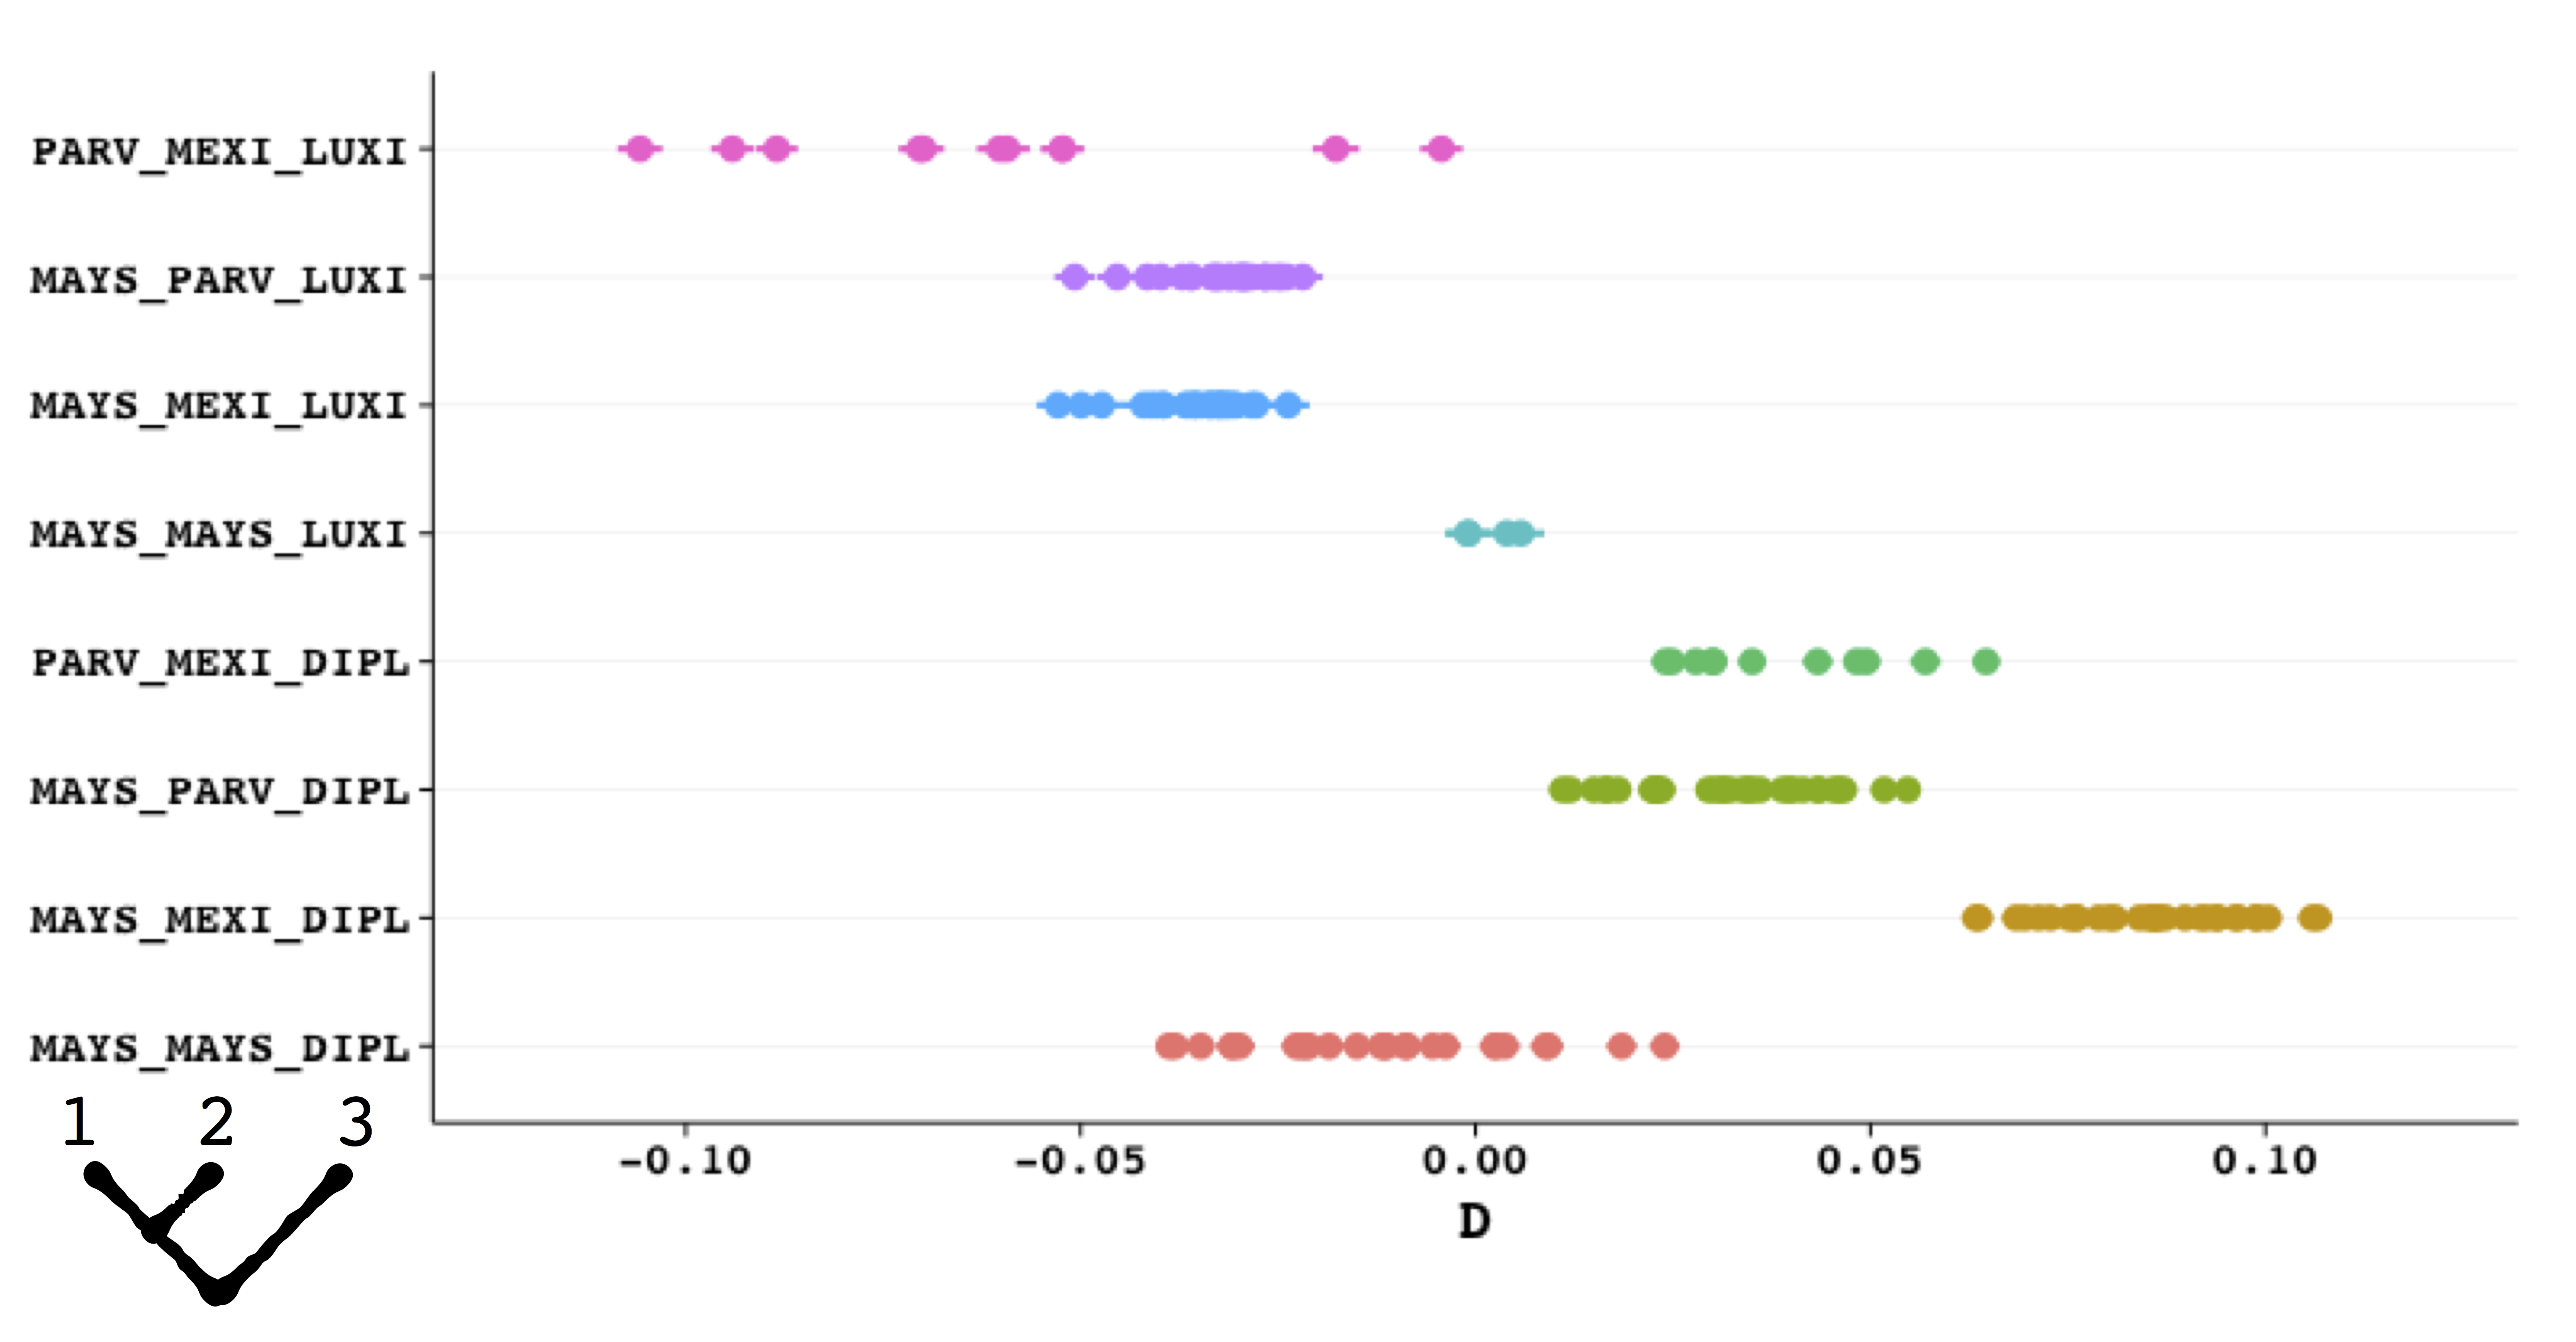
\includegraphics[width=0.8\textwidth]{abbas}
    \caption{Genome-wide evidence for admixture among \emph{Zea}. In the absence of admixture, taxa 1 and 2 on the tree should share similar numbers of derived alleles with taxa 3 due to the stochastic nature of incomplete lineage sorting.  Admixture leads to deviations from this expectation as measured by the D statistic \citep{green2010draft}. Negative values of D indicate admixture between taxa 1 and 3, while positive values indicate admixture between taxa 2 and 3.} 
\label{fig:abba}
\end{figure}

Speciation and divergence in \emph{Zea} is relatively recent, however, and an alternative explanation for at least some of these results is that polymorphisms found in ancestral populations continue to segregate in multiple taxa. 		
Simple estimates of the length of shared haplotypes expected to be unbroken by recombination over the $\sim$150,000-generation divergence time between \zm{} and \zl{} \citep{Ross-Ibarra2009a} suggest we might expect to see shared haplotypes of even several kb in length in low recombination regions of the genome (Figure \ref{fig:length}).

\begin{SCfigure}[][t]
  \centering
   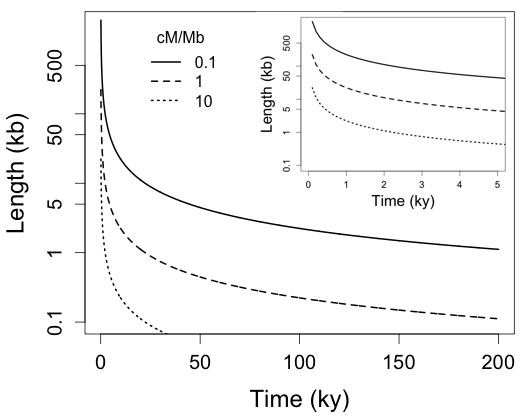
\includegraphics[width=0.6\textwidth]{length_vs_time2}
    \caption{Effect of recombination on the expected length of a shared chromosome segment vs. number of years since divergence or introgression.  Shown are three levels of recombination roughly representing high, average, and low recombination regions of the maize genome.}
\label{fig:length}
\end{SCfigure}

We will make use of both genotyping and whole-genome sequence data to test whether observed patterns of haplotype sharing among allopatric teosinte are consistent with recent introgression via maize or can be better explained by segregating ancestral polymorphism.
Although the limited sampling in \citet{Ross-Ibarra2009a} only identified shared haplotypes between \zm\ and \zl, maize is known to hybridize with all taxa in the genus.
Genome-wide genetic marker data do not currently exist for either \zd{} or its autotetraploid derivative \emph{Zea perennis} (hereafter, \emph{perennis}); we will sample 12 individuals from each of two accessions already available to us of both \zd{} and \emph{perennis} for genotyping using GBS. 
We will also generate full-genome sequence for one \zd{} (in addition to one current sequence -- see Preliminary Results) and an additional \zl{}.
These samples, combined with our other teosinte populations (\ref{sss:adaptive_intro} and \ref{sss:scale}), will provide a representative sample of all wild teosinte populations.
We will use window-based approaches \citep[e.g.,][]{martin2015evaluating} to estimate the size of putatively introgressed chromosomal segments from GBS data; these will be combined with more powerful haplotype-based analysis of full genome sequence data \citep{price2009}.  
Haplotypes shared between two teosinte as a result of gene flow via a maize intermediate will be of recent origin given the timing of maize domestication and subsequent range expansion. 
Recent introgression events will result in longer shared haplotypes (Figure \ref{fig:length}) and should be distinguishable from the genome-wide distribution of shared haplotype lengths as well as lengths predicted based on divergence time and local recombination rates.  
Estimates of local recombination rates will utilize either a 1cM-resolution map from maize \citep{wallace2014association} or a teosinte map under development in the Ross-Ibarra lab (see Potential Challenges).

We will complement the comparative analysis of teosinte with a survey of maize diversity data.
Although we cannot exhaustively test for the presence of putatively shared haplotypes in all of maize, we can survey publicly available data --- including GBS genotypes for more than $>4,000$ maize landraces \citep{Hearne2015} and whole genome sequence of more than 1000 diverse lines (\url{http://www.panzea.org/#!genotypes/cctl}) --- to search for such haplotypes in domesticated maize.

\paragraph{Preliminary Results}
\label{par:prelimII}
We have made arrangements with collaborators to assist in collection of maize, \zl\ and \zh\ from Guatemala.  The Ross-Ibarra and Hufford labs already have sufficient seed for all other samples for \ref{sss:bridge} and \ref{sss:scale}.

As part of a USDA grant on climate change to Drs. Ross-Ibarra and Hufford, we have sequenced more than 30 maize landrace accessions from across the range, including regions of sympatry with teosinte in Mexico and Guatemala. 
We have also recently sequenced multiple wild-collected \zp{} and a single \zd{} genome as part of another NSF-funded project.
These samples will prove invaluable for analysis of introgression and selection; comparison of these samples with published data corroborates earlier Sanger data suggesting admixture between allopatric teosinte (Figure \ref{fig:abba}).

\paragraph{Potential Challenges} \jri{need suggestions as to challenges here. one possibility: if we don't get lux/huehue seeds, what do we do? other potential pitfalls?}
No high-resolution genetic map currently exists for any teosinte, but we are currently working on producing such a map for \emph{parviglumis} as part of a different NSF project.
Evidence from comparisons among maize populations finds remarkable stability of the genetic map at a relatively coarse scale \citep{rodgers2015recombination} suggesting differences in the genetic map are unlikely to dramatically affect our estimates. 

\section*{Broader Impacts} \jri{ do we have a management plan? I think might be worth going to smaller font and adding a timeline. thoughts?}

Our efforts to broaden the impact of the research proposed here will begin within our groups through our commitment to effectively mentor volunteer undergraduate interns as well as graduate students and/or postdoctoral scholars funded by the project. Students and postdocs will receive one-on-one training from the investigators and senior personnel on laboratory, computational, and field research methods.  Mentees will also be encouraged and funded to present their work at scientific conferences.  Our groups have an excellent mentoring track record with four undergraduate students in the last five years publishing their work in scholarly journals and multiple underrepresented minorities participating in our research.

\jri{add something about undergraduate researchers in my lab?}

%\subsection*{ISU GK12 Fellowship Program}
%	
%In addition to the student and postdoc mentoring that will occur within our groups, as part of our broader impact activities each year one of our graduate students will participate in Iowa State University's GK12 Fellowship program (\emph{Symbi}; \url{http://www.gk12.iastate.edu/default.asp}; see attached letter of commitment). The selected graduate student will spend one full day each week in a middle or high school science classroom for the entire academic year of the Des Moines Public School District. This is the largest and most diverse school district in Iowa with over 50\% underrepresented minority student enrollment and over 70\% of students receiving free or reduced-cost lunch. The graduate student will introduce the K12 students to the scientific process through inquiry-based activities, relate the students’ science curriculum to real world examples, work with students on their science fair projects, and serve as a role model in a STEM profession. Furthermore, the graduate student will introduce students to his/her research project on hybridization and introgression in \emph{Zea}, a topic that is particularly well suited for teaching evolution in Iowa given the important role that maize plays in the Iowan economy. In introducing his/her dissertation research, the graduate student will engage Des Moines students in how research is conducted and provide STEM content professional training to his/her partner teacher.
%
%The GK12 Fellow will work with approximately 150 students on a regular weekly basis.  Student assessments from the ISU GK12 Fellowship Program have shown that a significant number of students like science more after having a GK Fellow in the classroom.  Teachers report that having a GK12 Fellow in their classroom is excellent professional development.  The PI will also visit the classroom and will support the selected graduate student in their development of appropriate material for the K12 audience.

\subsection*{US-Mexico Exchange Program}
	
Finally, we will establish a student exchange program between the Eguiarte Laboratory at UNAM in Mexico and the Hufford and Ross-Ibarra Laboratories in the United States. The Ross-Ibarra Laboratory has run an NSF-supported, US-Mexico exchange program for the last four years.  
All of the exchange students involved in the program have continued on to additional graduate work, and two have earned authorship on published or forthcoming papers from their internship.  
We will build upon the success of this program.
Each year \jri{is this correct? every year?} a graduate or undergraduate student from the Eguiarte group spending 2-3 months in either the Hufford or Ross-Ibarra Laboratory learning GBS methodology and/or population genomic analysis, and a student from the Hufford or Ross-Ibarra Laboratories will travel to Mexico to participate in sample collection trips and to obtain expertise in common garden field experiments. 
This exchange will build capacity in all groups involved and will provide students with valuable international research experience.  

Senior Personnel Claudia Calder\'{o}n has previously led international student research trips and will assist in preparing students from both the United States and Mexico for the exchange program. A survey will be given to both exchange students and faculty in order to gauge expectations prior to the trip and facilitate collaborations amongst the labs.  The survey will also assess students' knowledge and preconceived ideas  regarding their travel destinations.  A meeting (online or face-to-face) with the cohort of students traveling will help address these pre-conceptions and reduce cultural misunderstandings.  Suggestions will be given to students of how to prepare before the trip (visa, immigration requirements) and how to communicate with their peers and others during their exchange.  Students will be given information regarding the facilities where they will be staying, transportation to be used, food and water safety, the availability of telecommunications and general safety guidelines.

\required{Results From Prior NSF Support} \jri{i edited both rare alleles and the centromere grant. include one or both as you see fit}

% 5 pages or fewer of the 15 pages for entire description document.
% include results from NSF grants received in the past 5 years.
% If supported by more than one grant, choose the most relevant one.

% For each grant, include: 
%	(a) NSF award number, amount, dates of support 
%	(b) The title of this project
%	(c) Publications resulting from this research
%	(d) Summary of the results of the completed work
%	(e) A brief description of data samples available and other research products not described 	      elsewhere
%	(f) For renewed support, a description of the relationship between the completed and 			      proposed work

% Due to space limitations, it is often advisable to use citations rather
% than putting the titles of the publications in the body 
% of this section

\subsection*{NSF \#1404974: US-Mexico Planning Visit and Workshop to Assess the Genomic Basis of Local Adaptation in Maize} 
\$34,650. 09/01/14-08/31/15. PI Matthew Hufford, co-PI J. Ross-Ibarra, G. Coop, Senior Personnel S. Flint-Garcia, Collaborators R. Sawers and A. Cibrian-Jaramillo
\par\noindent{\bf Intellectual merit} Through planning meetings and a phenotyping workshop in Mexico, this project has established a new international collaboration and laid the foundation for work proposed in a pending Plant Genome Research Program proposal. Planning meetings helped coordinate generation of preliminary data described in this proposal and the phenotyping workshop transferred high-throughput methods across our research groups.
\par\noindent{\bf Broader impacts} Participants in the  workshop included graduate students and postdoctoral scholars from the US and Mexico, providing STEM training and international scientific experience.
\par\noindent{\bf Publications} Funding is for organizational purposes; no publications are expected from this award.

\subsection*{NSF \#1238014: Biology of Rare Alleles in Maize and Its Wild Relatives}
\$13,311,185 (\$2,368,767 to Ross-Ibarra), 05/15/13-04/30/18. PI Edward Buckler, co-PIs P. Bradbury, J. Doebley,  S. Flint-Garcia, J. Holland,  S. Mitchell, J. Ross-Ibarra, Q. Sun.
\par\noindent{\bf Intellectual merit} In the first two years of this proposal we have developed imputation approaches, found evidence for the importance of deleterious variants in determining heterosis, documented copy number variation in natural teosinte populations, and found population genetic evidence suggesting the importance of demography in patterning purifying selection across the genome. 
\par\noindent{\bf Broader impacts} The project so far has included 4 postdoctoral and 1 graduate trainees in the Ross-Ibarra lab. and the project GBS workshop and museum exhibit continue to be popular. 
\par\noindent{\bf Publications} \citet{tiffin2014advances, Takuno15062015, da2015origin, hake2015genetic, makarevitch2015transposable} 
%\subsection*{NSF \#0922703: Functional Genomics of Maize Centromeres}
%\$5,008,031 (\$754,409 to Ross-Ibarra). 09/01/09-08/31/14. PI Kelly Dawe, co-PIs J. Birchler, J. Jiang, G. Presting, J. Birchler, J. Ross-Ibarra
%\par\noindent{\bf Intellectual merit} Centromeres are regions of the genome that organize and regulate chromosome movement, yet the biology of centromeres remains poorly understood. Co-PI Ross-Ibarra's group focused in particular on the evolutionary genetics of centromeres, demonstrating the lability of centromere tandem repeats but also showing little evidence in maize for coevolution between centromere sequence and kinetochore proteins. \par\noindent{\bf Broader impacts}  Co-PI Ross-Ibarra  established a succesful international student exchange program. Former trainees on the grant include Dr. Matthew Hufford (PI on the current grant).\
%\par\noindent{\bf Publications} \citet{Shi2010a, Chia2012a, Fang2012, Hufford2012, Hufford2012b, Hufford2013, Melters2013a, Kanizay2013, Pyhajarvi2013}